\chapter{Remote Method Invocation}
\section{Overview}
In modern, large distributed systems, nodes can be running in processes on several different physical machines. Using the Java Remote Method Invocation this can be done opaquely from the user. 

The Java RMI makes this possible. 

\section{Java RMI}
\subsection{Java Virtual Machine}
The Java Virtual Machine is a component that can execute Java bytecode. It is has an implementation on almost every platform and makes it possible to reuse your code on all these platforms. It JIT compiles the code to enable garbage collection and runtime code verification, so that programmer errors and safety isssues is avoided.
Java bytecode and the JVM is analogous to Microsoft's .NET managed code and CLR (Common Language Runtime).

\subsection{Remote Method Invocation}

\subsection{Serialization}
To be able to send data to another component / computer, Java RMI needs to serialize the data when it is send and then deserialize it when it is received. 
Serialization means to convert some data into sequence of bytes that holds the original values and information on the source eg what kind of object it is. It should also be possible to convert it back into the original data at any time (deserialize). This concept is often used when data is saved into a file or database or when data is transferred over a network.

\subsection{The RMI Registry}

\section{Leader election}
\subsection{Overview}

\subsection{Leader Election}

\subsection{Bully Election}
The bully election algorithm basically elects the process with biggest process id as the new leader when the old leader is terminated. 
If a process takes contact to the leader and doesn't get a response, it will then start a leader election by asking all processes with an id greater than its own, if they will be the leader. These processes will then reply if they are active that they will take over by continuing the algorithm. 

If a process doesn't get an answer, then it is elected as the new leader and will state this to all other processes.

This algorithm is very ineffective because you will quickly get a very high number of requests when all processes must ask all other processes with a higher id.

\subsection{Ring Election}



%Picture:
%\begin{center}
%	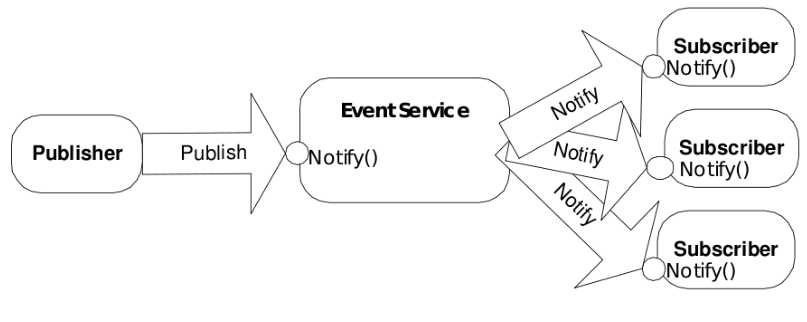
\includegraphics[width=\textwidth]{PublishSubscribe_Pattern.png}
%	\captionof{figure}{Sublish/Subscribe pattern}
%\end{center}


